\documentclass[12pt, a4paper]{article}
\usepackage{amsmath}
\usepackage{enumitem}
\usepackage{float}
\usepackage[left=2cm, right=2cm, top=2cm, bottom=2cm]{geometry}
\usepackage{graphicx}
\usepackage[colorlinks, urlcolor=blue]{hyperref}
\usepackage{minted}
\usepackage{xeCJK}

\renewcommand\arraystretch{1.5}
\setCJKmainfont[AutoFakeBold=1.5]{新細明體}
\setlength{\parindent}{0pt}

\setminted{
  frame=single,
  tabsize=2,
}

\title{
  \vspace{-1cm}
  Network Administration/System Administration\\
  (NTU CSIE, Spring 2024)\\
  Homework \#11 - Nginx
}
\author{\Large B12902110 呂承諺}

\begin{document}
  \maketitle

  \section*{Web Terminology}
  \begin{enumerate}
    \item

    \item

    \item

    \item

    \item
  \end{enumerate}

  \section*{Web Server Configurations}
  \begin{enumerate}[resume]
    \item \textbf{Steps}
    \begin{enumerate}[label=(\arabic*)]
      \item Run the following commands.
      \begin{Verbatim}[frame=single]
$ cp -r /tmp2/nasa-hw11 /tmp2/b1290110
$ cd /tmp2/b12902110/nasa-hw11
$ qemu-img create -f qcow2 disk0.qcow2 20G
      \end{Verbatim}
      \item Create \verb|/tmp2/b12902110/nasa-hw11/run_vm.sh| as the following.
      \inputminted[fontsize=\scriptsize]{shell}{run_vm.sh}
      \item Boot up the VM, connect to it via QEMU's VNC, and follow the Debian installation guide. After the installation finished, reboot into the VM.
      \item Configure sudo as the root user.
      \begin{Verbatim}[frame=single]
$ su
# apt install -y sudo
# usermod -aG sudo b12902110
      \end{Verbatim}
      \item Re-login as user b12902110. Install the necessary package for our
      web server.
      \begin{Verbatim}[frame=single]
$ sudo apt install -y nginx
      \end{Verbatim}
      \item Start the nginx service.
      \begin{Verbatim}[frame=single]
$ sudo systemctl start nginx.service
      \end{Verbatim}
    \end{enumerate}

    \textbf{Result}

    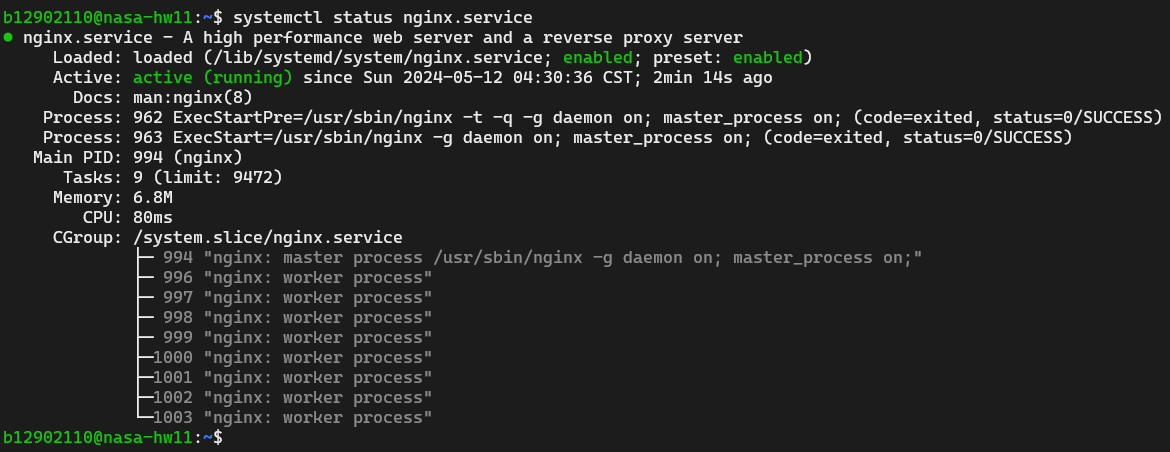
\includegraphics[width=0.9\textwidth]{6_result.png}

    \textbf{References}
    \begin{itemize}
      \item \href{https://www.linuxquestions.org/questions/linux-newbie-8/command-usermod-not-found-385901/}{command usermod not found}
    \end{itemize}

    \item \textbf{Steps}
    \begin{enumerate}[label=(\arabic*)]
      \item Install \verb|ufw|.
      \begin{Verbatim}[frame=single]
$ sudo apt install -y ufw
      \end{Verbatim}
      \item Configure firewall rules with the following commands.
      \begin{Verbatim}[frame=single]
$ sudo ufw default deny
$ sudo ufw allow 22
$ sudo ufw allow 80
$ sudo ufw allow 443
$ sudo ufw enable
      \end{Verbatim}
    \end{enumerate}

    \textbf{Result}

    This part is done after the last problem, so we have more services than an HTTP
    and an SSH service.

    In the QEMU console, add another port forwarding rule: 11088 on the host to
    8888 on the VM.
    \begin{Verbatim}[frame=single]
(qemu) hostfwd_add tcp::11088-:8888
    \end{Verbatim}

    Therefore, we have 4 port forwarding rules.

    \begin{tabular}{|ll|}
      \hline
      \textbf{Source} & \textbf{Destination} \\\hline
      ws2.csie.ntu.edu.tw:11022 & nasa-hw11:22 \\
      ws2.csie.ntu.edu.tw:11080 & nasa-hw11:80 \\
      ws2.csie.ntu.edu.tw:11043 & nasa-hw11:443 \\
      ws2.csie.ntu.edu.tw:11088 & nasa-hw11:8888 \\
      \hline
    \end{tabular}

    All of the 4 ports has a service running on it.

    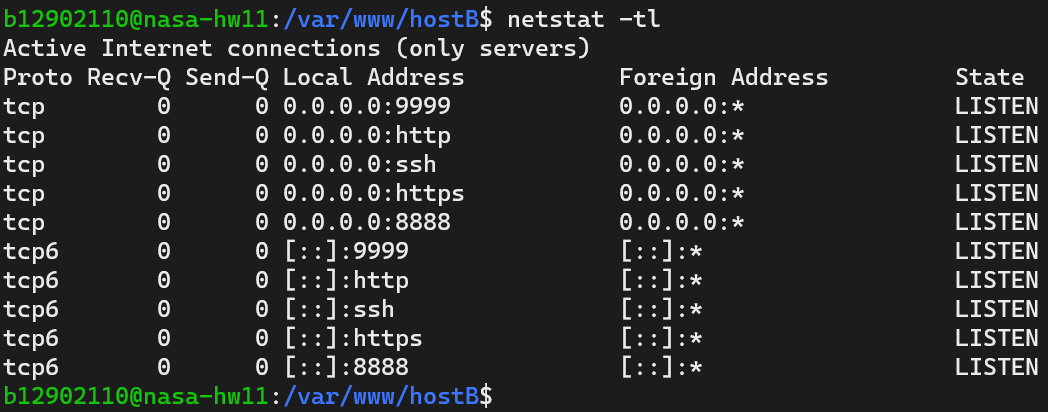
\includegraphics[width=0.7\textwidth]{7_netstat.png}

    However, only ports 22, 80, and 443 are accessible from outside
    the VM.

    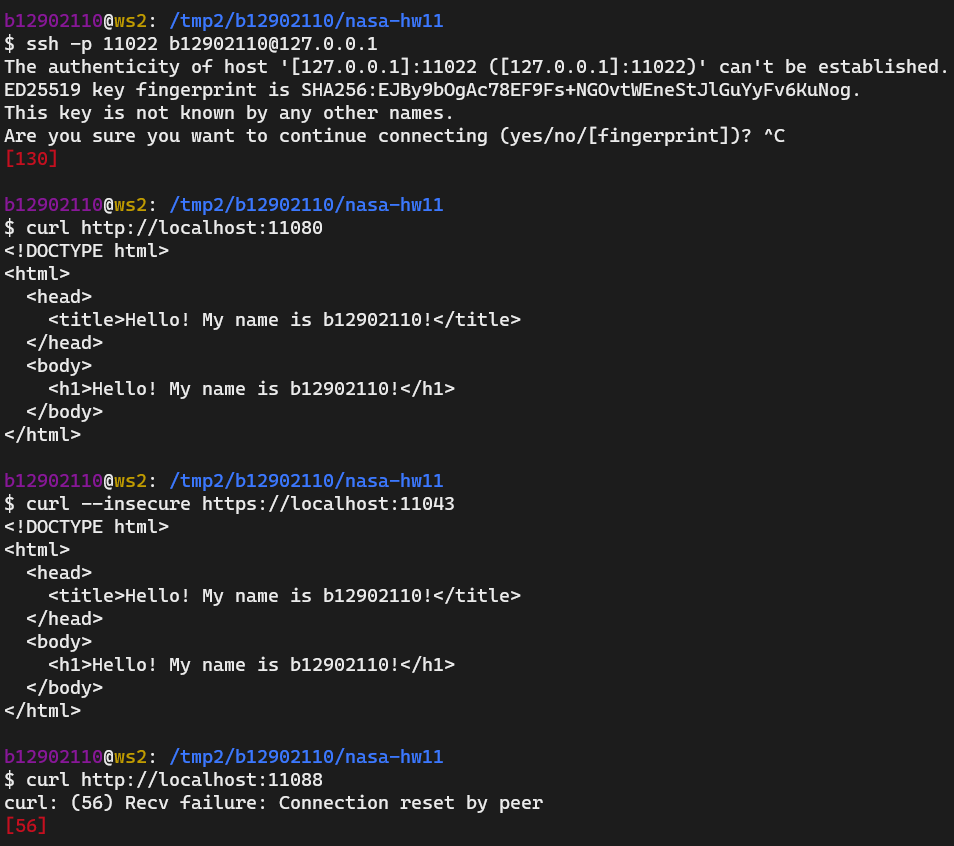
\includegraphics[width=0.7\textwidth]{7_access.png}

   \textbf{References}
   \begin{itemize}
     \item \href{https://www.digitalocean.com/community/tutorials/opening-a-port-on-linux}{How To Open a Port on Linux  | DigitalOcean}
     \item \href{https://www.digitalocean.com/community/tutorials/how-to-set-up-a-firewall-with-ufw-on-ubuntu}{How to Set Up a Firewall with UFW on Ubuntu  | DigitalOcean}
   \end{itemize}

    \item \textbf{Steps}

    Create \verb|/var/www/html/index.html| as the following.
    \inputminted{html}{server/var/www/html/index.html}

    \textbf{Result}

    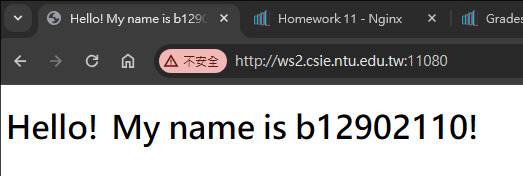
\includegraphics[width=0.5\textwidth]{8_result.png}

    \item \textbf{Steps}
    \begin{enumerate}[label=(\arabic*)]
      \item Add the following \verb|location| block into
      \verb|/etc/nginx/sites-available/default|.
      \begin{Verbatim}[frame=single]
server {
  ...

  location ~ ^/~(.*?)/(.*) {
    alias /home/$1/htdocs/$2;
  }

  ...
}
      \end{Verbatim}
      \item Run the following commands.
      \begin{Verbatim}[frame=single]
$ chmod 755 /home/b12902110
$ mkdir /home/b12902110/htdocs
      \end{Verbatim}
      \item Create \verb|/home/b12902110/htdocs/index.html| as the following.
      \inputminted{html}{server/home/b12902110/htdocs/index.html}
      \item Reload the nginx service.
      \begin{Verbatim}[frame=single]
$ sudo systemctl reload nginx.service
      \end{Verbatim}
    \end{enumerate}

    \textbf{Result}

    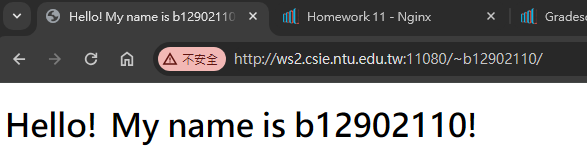
\includegraphics[width=0.6\textwidth]{9_result.png}

    \textbf{References}
    \begin{itemize}
      \item \href{https://stackoverflow.com/questions/42605637/nginx-user-public-home-without}{nginx user public home without ~ - Stack Overflow}
      \item \href{https://nginx.org/en/docs/beginners_guide.html}{Beginner's Guide}
      \item \href{https://nginx.org/en/docs/http/ngx_http_core_module.html}{Module ngx\_http\_core\_module}
    \end{itemize}

    \item \textbf{Steps}
    \begin{enumerate}[label=(\arabic*)]
      \item Add the following \verb|location| block into
      \verb|/etc/nginx/sites-available/default|.
      \begin{Verbatim}[frame=single]
server {
  ...

  location = /secret.html {
    allow 192.168.28.0/24;
    deny all;
  }

  ...
}
      \end{Verbatim}

      \item Reload the nginx service.
      \begin{Verbatim}[frame=single]
$ sudo systemctl reload nginx.service
      \end{Verbatim}
    \end{enumerate}

    \textbf{Result}

    Before restriction:

    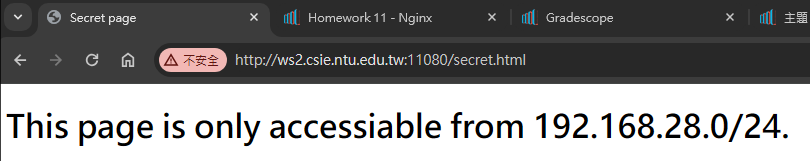
\includegraphics[width=0.6\textwidth]{10_result_before.png}

    After restriction:

    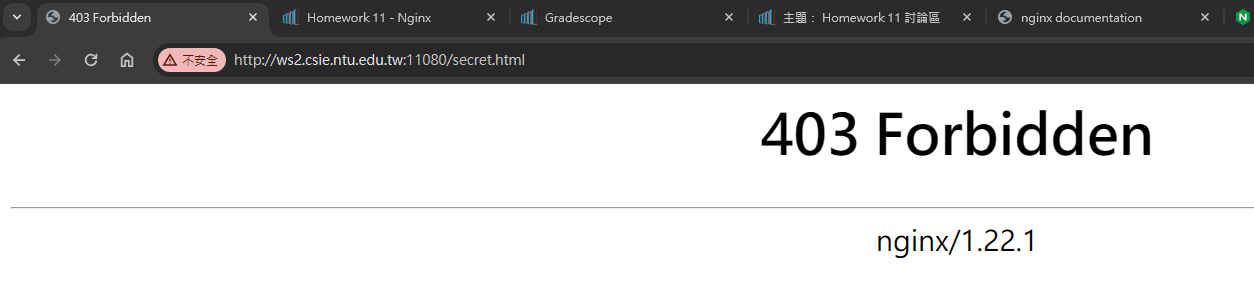
\includegraphics[width=0.8\textwidth]{10_result_after.png}

    \textbf{References}
    \begin{itemize}
      \item \href{https://nginx.org/en/docs/http/ngx_http_access_module.html}{Module ngx\_http\_access\_module}
    \end{itemize}

    \item \textbf{Steps}

    View the last few lines of \verb|/var/log/nginx/access.log|/
    \begin{Verbatim}[frame=single]
$ sudo tail /var/log/nginx/access.log
    \end{Verbatim}

    \textbf{Result}

    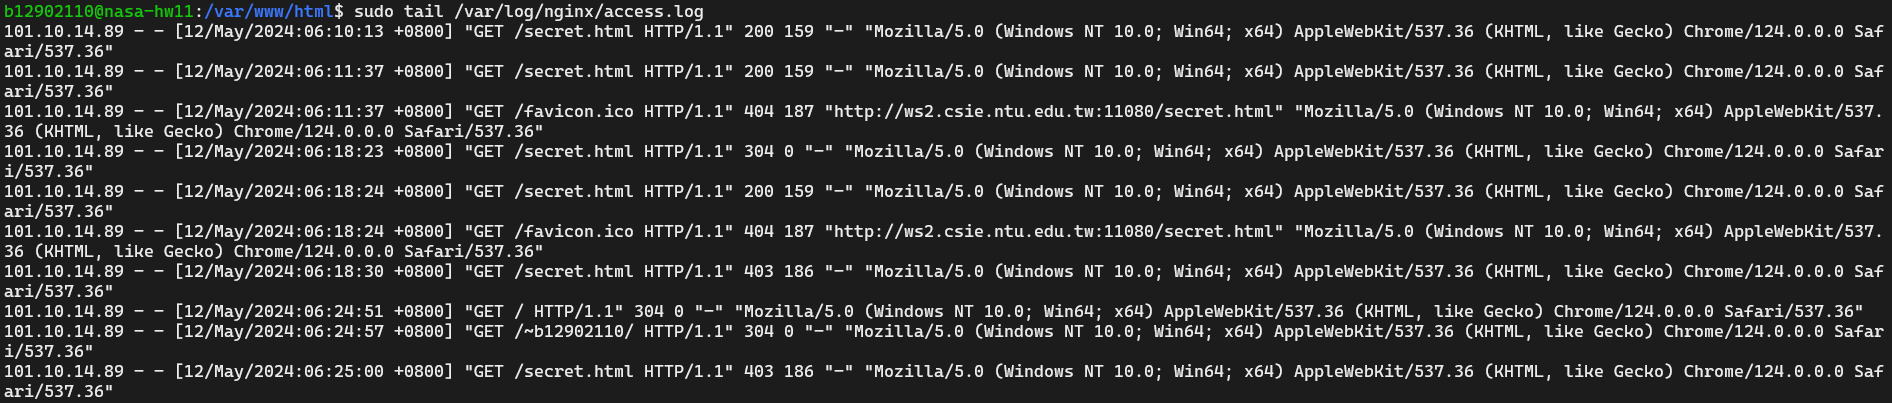
\includegraphics[width=0.93\textwidth]{11_result.png}

    \textbf{References}
    \begin{itemize}
      \item \href{https://docs.nginx.com/nginx/admin-guide/monitoring/logging/}{Configuring Logging | NGINX Documentation}
    \end{itemize}

    \item
    \begin{enumerate}
      \item

      \item

      \item \textbf{Steps (Server)}
      \begin{enumerate}[label=(\arabic*)]
        \item Create CA key and certificate.
        \begin{Verbatim}[frame=single, fontsize=\footnotesize]
$ openssl req -new -x509 -noenc -days 365000 -keyout ca-key.pem \
    -out ca-cert.pem

...

-----
Country Name (2 letter code) [AU]:TW
State or Province Name (full name) [Some-State]:Taiwan
Locality Name (eg, city) []:
Organization Name (eg, company) [Internet Widgits Pty Ltd]:NTU CSIE
Organizational Unit Name (eg, section) []:
Common Name (e.g. server FQDN or YOUR name) []:
Email Address []:
        \end{Verbatim}
        \item Create server key and certificate request.
        \begin{Verbatim}[frame=single, fontsize=\footnotesize]
$ openssl req -new -noenc -keyout server-key.pem -out server-req.pem

...

-----
Country Name (2 letter code) [AU]:TW
State or Province Name (full name) [Some-State]:Taiwan
Locality Name (eg, city) []:
Organization Name (eg, company) [Internet Widgits Pty Ltd]:NTU CSIE
Organizational Unit Name (eg, section) []:
Common Name (e.g. server FQDN or YOUR name) []:nasa-hw11
Email Address []:
        \end{Verbatim}
        \item Sign the server certificate.
        \begin{Verbatim}[frame=single]
$ openssl x509 -req -days 365000 -in server-req.pem \
    -out server-cert.pem -CA ca-cert.pem -CAkey ca-key.pem
Certificate request self-signature ok
subject=C = TW, ST = Taiwan, O = NTU CSIE, CN = nasa-hw11
        \end{Verbatim}

        \item Install the certificates to \verb|/etc/nginx|.
        \begin{Verbatim}[frame=single]
$ sudo cp server-key.pem server-cert.pem /etc/nginx
$ sudo chown www-data:www-data /etc/nginx/server-key.pem
        \end{Verbatim}
        \item Configure the following \verb|server| settings in\\
        \verb|/etc/nginx/sites-available/default|.
        \begin{Verbatim}[frame=single]
server {
  ...

  listen 443 ssl default_server;
  listen [::]:443 ssl default_server;
  ssl_certificate server-cert.pem;
  ssl_certificate_key server-key.pem;

  ...
}
        \end{Verbatim}
        \item Reload the nginx service.
        \begin{Verbatim}[frame=single]
$ sudo systemctl reload nginx.service
        \end{Verbatim}
      \end{enumerate}

      \textbf{Steps (Windows Client)}

      Run \verb|certmgr.msc|, and install \verb|ca-cert.pem| to
      ``Trusted Root Certification Authorities".

      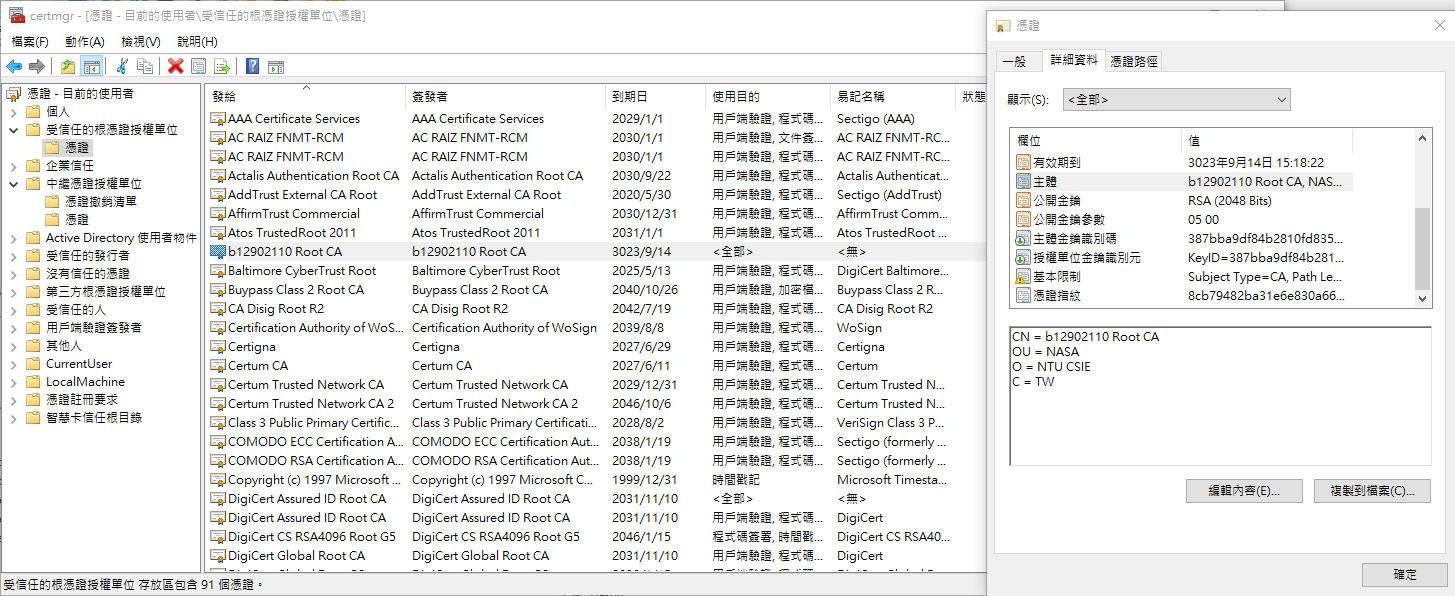
\includegraphics[width=0.87\textwidth]{12-c_certmgr.png}

      \textbf{Result}

      Certificates:

      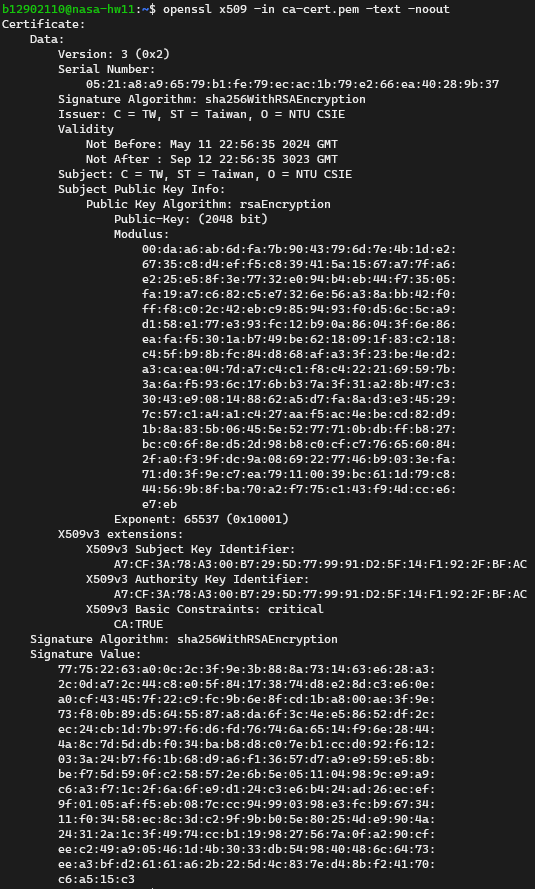
\includegraphics[width=0.43\textwidth]{12-c_ca-cert.png}
      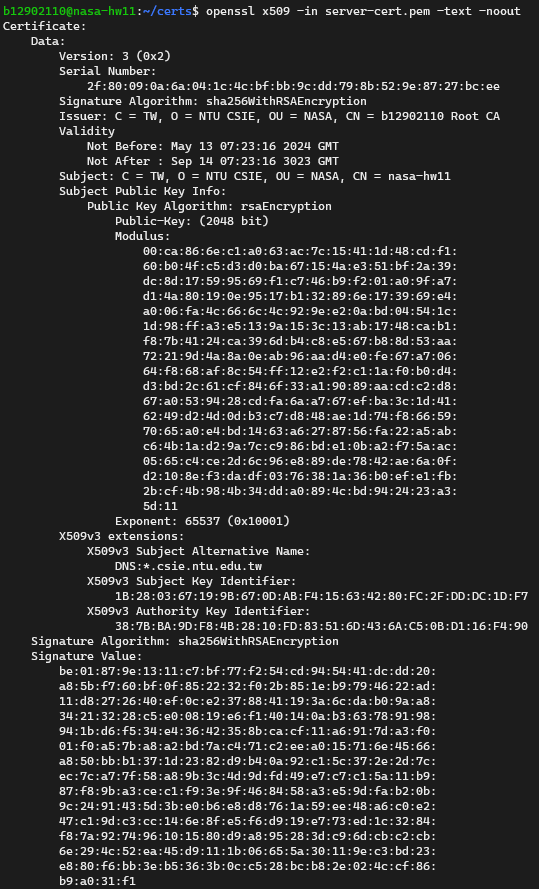
\includegraphics[width=0.43\textwidth]{12-c_server-cert.png}

      Browser:

      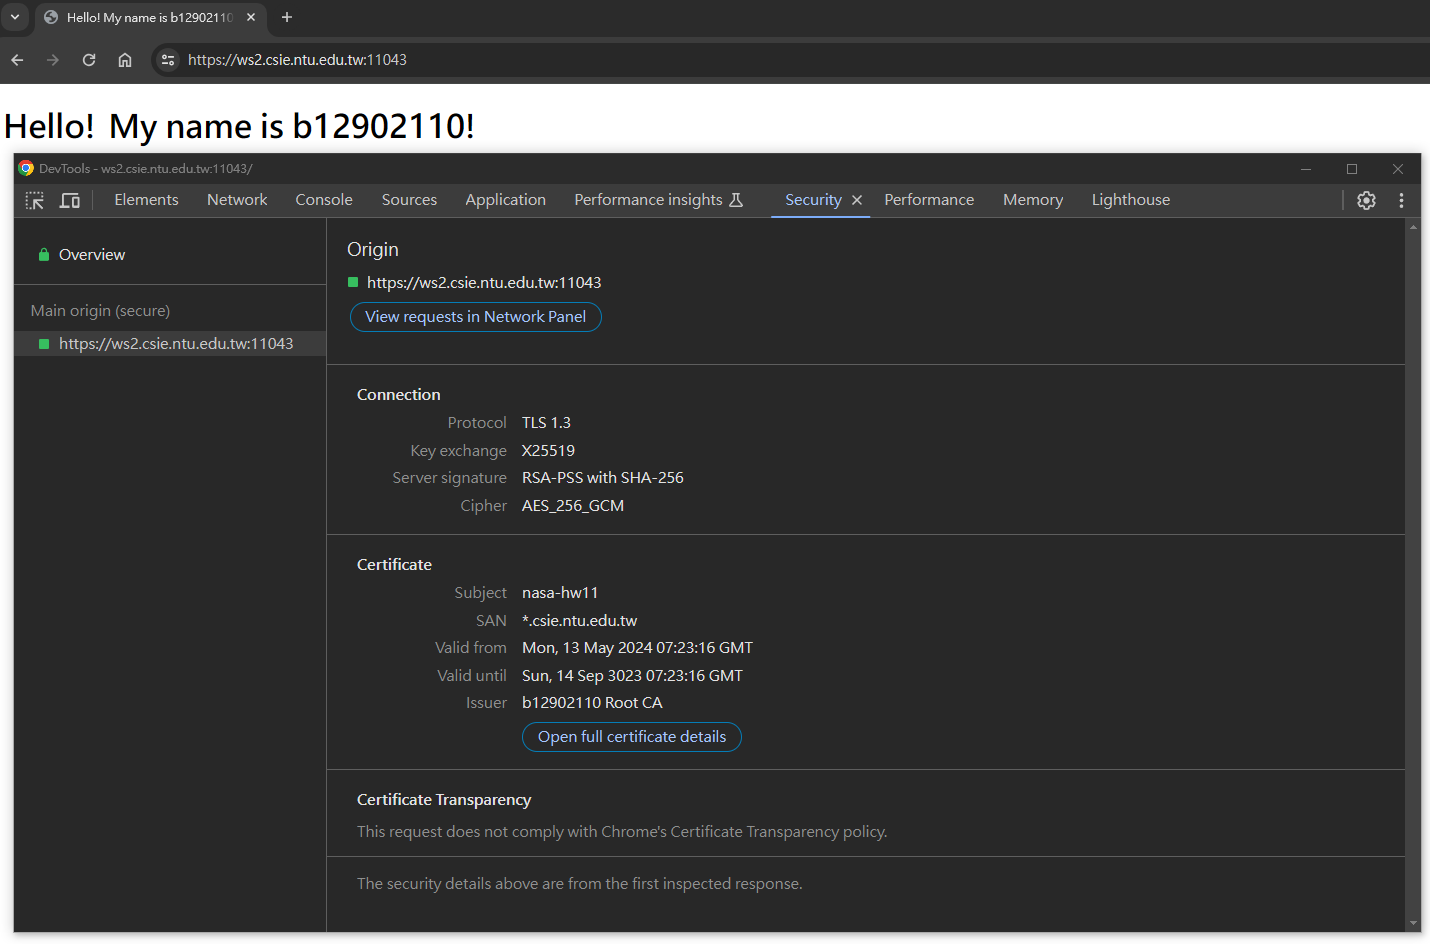
\includegraphics[width=0.6\textwidth]{12-c_browser.png}

      Since we're using NAT here, it still shows up as insecure due to\\
      \verb|NET::ERR_CERT_COMMON_NAME_INVALID|.

      \textbf{References}
      \begin{itemize}
        \item \href{https://mariadb.com/docs/server/security/data-in-transit-encryption/create-self-signed-certificates-keys-openssl/}{Create Self-Signed Certificates and Keys with OpenSSL — MariaDB Documentation}
        \item \href{https://www.openssl.org/docs/man3.0/man1/openssl-req.html}{/docs/man3.0/man1/openssl-req.html}
        \item \href{https://www.openssl.org/docs/man3.0/man1/openssl-x509.html}{/docs/man3.0/man1/openssl-x509.html}
      \end{itemize}

    \end{enumerate}
  \end{enumerate}

  \section*{Reverse Proxy}
  \begin{enumerate}[resume]
    \item \textbf{Steps}
    \begin{enumerate}[label=(\arabic*)]
      \item Create \verb|/etc/nginx/sites-available/hostA| as the following.
      \inputminted{nginx}{server/etc/nginx/sites-available/hostA}
      \item Create \verb|/etc/nginx/sites-available/hostB| as the following.
      \inputminted{nginx}{server/etc/nginx/sites-available/hostB}
      \item Enable both \verb|hostA| and \verb|hostB|.
      \begin{Verbatim}[frame=single]
$ sudo ln -s /etc/nginx/sites-available/hostA \
    /etc/nginx/sites-enabled/hostA
$ sudo ln -s /etc/nginx/sites-available/hostB \
    /etc/nginx/sites-enabled/hostB
      \end{Verbatim}
      \item Create \verb|/var/www/hostA/index.html| as the following.
      \inputminted{html}{server/var/www/hostA/index.html}
      \item Create \verb|/var/www/hostB/index.html| as the following.
      \inputminted{html}{server/var/www/hostB/index.html}
      \item Add \verb|/hostA| and \verb|/hostB| location blocks to
      \verb|/etc/nginx/sites-available/default|.
      \begin{Verbatim}[frame=single]
server {
  ...

  location /hostA {
    proxy_pass http://127.0.0.1:8888/;
  }

  location /hostB {
    proxy_pass http://127.0.0.1:9999/;
  }

  ...
}
      \end{Verbatim}
      \item Reload the nginx service.
      \begin{Verbatim}[frame=single]
$ sudo systemctl reload nginx.service
      \end{Verbatim}
    \end{enumerate}

    \textbf{Result}

    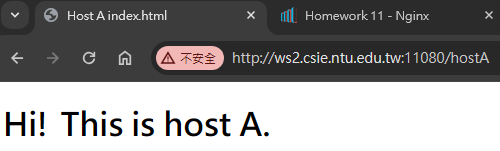
\includegraphics[width=0.45\textwidth]{13_hostA.png}
    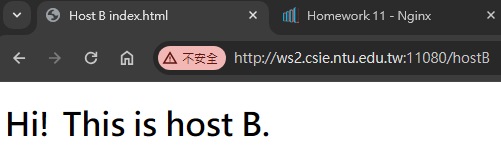
\includegraphics[width=0.45\textwidth]{13_hostB.png}

    \textbf{References}
    \begin{itemize}
      \item \href{https://nginx.org/en/docs/beginners_guide.html}{Beginner's Guide}
      \item \href{https://nginx.org/en/docs/http/ngx_http_proxy_module.html}{Module ngx\_http\_proxy\_module}
    \end{itemize}
  \end{enumerate}
\end{document}
